\documentclass{cv}

% Font
\usepackage{lmodern}
	\renewcommand*\familydefault{\sfdefault}
\usepackage[T1]{fontenc}

% Spacing between lines within a paragraph
\renewcommand{\baselinestretch}{1.1}

% Utilities
\usepackage{subfig}
\usepackage{enumitem}
\usepackage{siunitx}
\usepackage{graphicx}

% Metadata
\usepackage{hyperref}
\hypersetup{
	pdfinfo={
		Title = {Curriculum Vitae},
		Subject = {Curriculum Vitae - IoT version (09/11/2019)},
		Author = {Daniel Ríos Linares},
		Keywords = {CV, Industrial, Electronic, Engineer, IoT, Programming, CAD},
		Creator = {LaTeX with CV class},
		Producer = {TeXLive pdfTeX},
		Version = {IoT (09/11/2019)}
		}
	}

% Colors
\definecolor{spirodiscoball}{rgb}{0.06, 0.75, 0.99}

% Sidebar

	% Main
	\colorlet{side@main@text}{white}
	\colorlet{side@main@bkgd}{spirodiscoball!85!white}

	% Sections
	\colorlet{side@sect@text}{white}
	\colorlet{side@sect@bkgd}{spirodiscoball!90!black}
	
	% General info
	\colorlet{side@info@text}{white}
	\colorlet{side@info@icon}{white}
	
	% Goals
	\colorlet{side@goal@text}{white}
	
	% Interests
	\colorlet{side@inte@text}{white}
	
	% Languages
	\colorlet{side@lang@text}{white}
	\colorlet{side@lang@empt}{gray}
	\colorlet{side@lang@fill}{lime}
	
		
	% Dial
	\colorlet{side@dial@text}{white}
	\colorlet{side@dial@empt}{gray}
	\colorlet{side@dial@fill}{lime}
	\colorlet{side@dial@bubb}{white}

% Body

	% Main
	\colorlet{body@main@text}{black!95}
	\colorlet{body@main@bkgd}{lightgray!1!white}
	
	% Sections
	\colorlet{body@sect@text}{black!95}
	
	% Bullet
	\setlist[itemize,1]{label=\color{cyan}$\blacktriangleright$}

% Text

	% Tiers
	\colorlet{tier@epc}{lime}
	\colorlet{tier@max}{violet}
	\colorlet{tier@med}{blue}
	\colorlet{tier@min}{black}

% Tooltips

	% Tiers
	\colorlet{tooltip@bkg}{cyan!20}
	\colorlet{tooltip@frm}{black!80}

\def\tooltipPython{\parbox{112mm}{
	\textcolor{blue}{Python} \hfill see GitHub 
\includegraphics[height=4mm]{resources/images/logos-circle/github.pdf} \\[3mm]
	· Familiarized with CPython 2.7/3.6+ (weekly basis since 2016) \\
	· Frequent visitor of PyCon online \\
	· Mainly OOP and concurrent approach \\
	· Favourite use: tedious tasks automation \\[2mm]
	· Basic libraries (\texttt{Numpy}, \texttt{Scipy}, \texttt{Sympy}) \\
	· Personal libraries when needed (\texttt{python-library}, see GitHub) \\
	· Python/C API wrapping: C subroutines (Instant/SWIG) \\
	· Tensorflow \\
	· Fortran90 wrapping: F2Py and C extend \\
	· Numerical computing (sped-up by C and Fortran90) \\
	· GUI design: proficiency in \texttt{PyQt5}+\texttt{MatPlotLib} \\
	· Graphics: svg, pdf automation \\
	· Format parsing: used for MathCAD, SAPWin and TikZ \\
	· Data manipulation: ranging from csv and SQL to wav \\
	· Website data extraction (\texttt{requests} and \texttt{SeleniumHQ}) \\
	· Cloud storage (Dropbox API, Mega.nz, Google drive) \\
	· Mouse events, keystrokes and remapping (\texttt{win32api} for Windows) \\
	· OS interaction \texttt{pywinauto} (Windows), \texttt{pyautogui} (Linux) \\
	· Real-time screen monitoring and control of virtual peripheral hardware
	}}

\def\tooltipSolidWorks{\parbox{110mm}{
	\textcolor{blue}{SolidWorks} \hfill see GrabCAD 
\includegraphics[height=4mm]{resources/images/logos-circle/grabcad.pdf} \\[3mm]
	· Plastic part design
	\begin{figure}[H]
		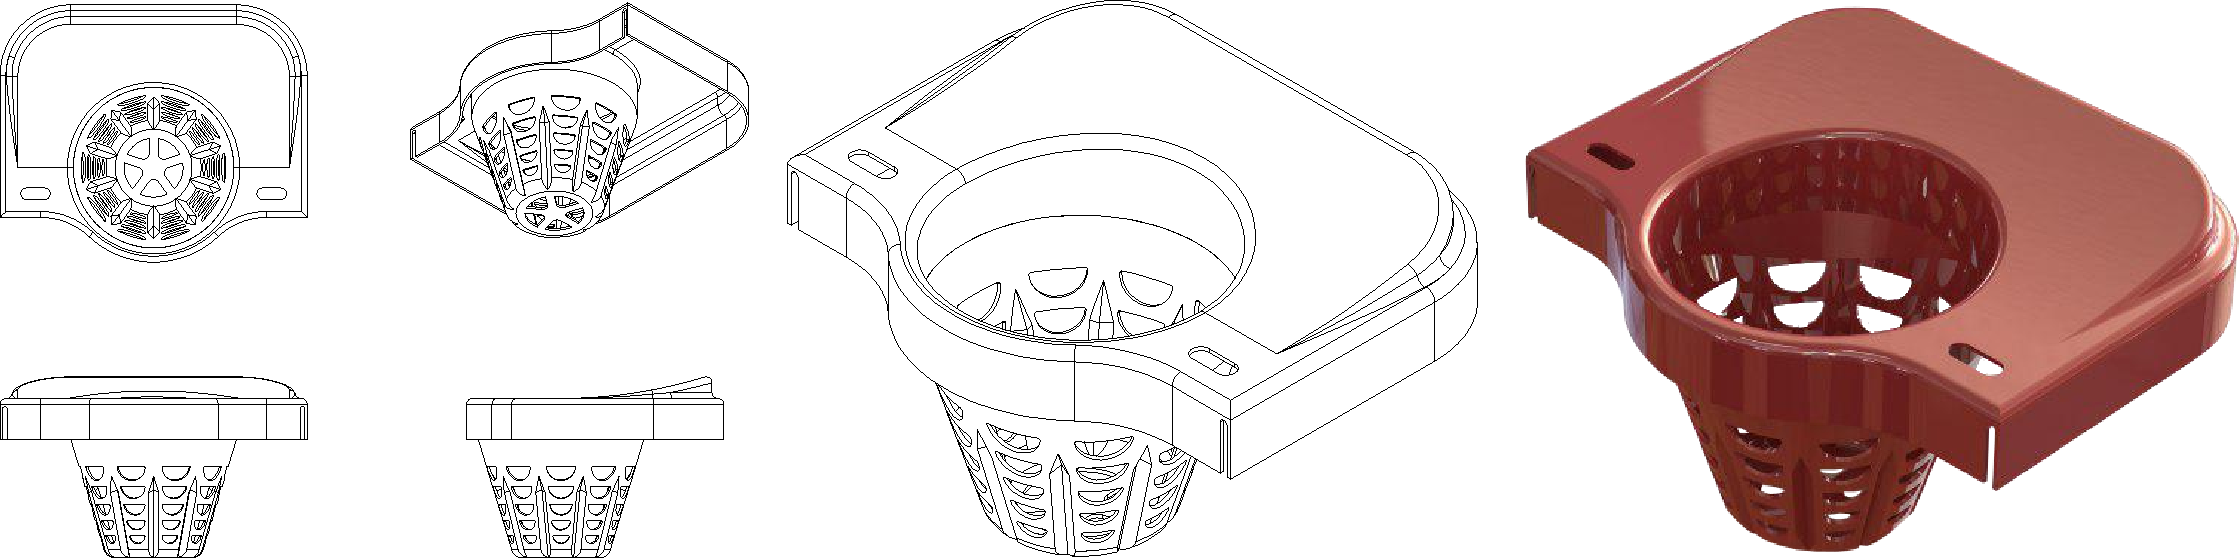
\includegraphics[width = 110mm]{resources/images/projects/solidworks/Mop_Wringer.pdf} \\[1mm]
		\centering\small Mop wringer (SolidWorks)
	\end{figure}
	}}

\def\tooltipRTOS{\parbox{110mm}{
	\textcolor{blue}{RTOS} \\[3mm]
	· Espressif ESP8266/ESP32
	}}

\def\tooltipSBC{\parbox{110mm}{
	\textcolor{blue}{Single-board computers} \\[3mm]
	· Raspberry Pi 3B+
	· pcDuino3
	}}

\def\tooltipThreeDPrinting{\parbox{110mm}{
	\textcolor{blue}{3D Printing (Fused Deposition Manufacturing)} \\[3mm]
	· Reparations
	\begin{figure}[H]
		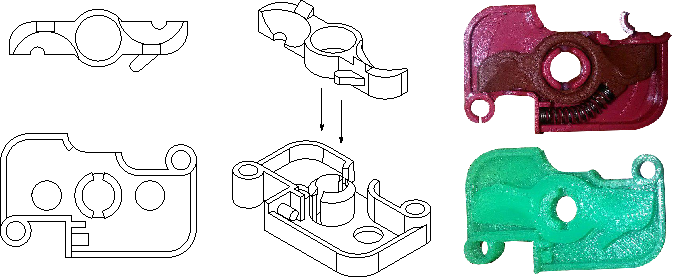
\includegraphics[width = 110mm]{resources/images/projects/solidworks/European_Plug_Socket_Cover.pdf} \\[1mm]
		\centering\small European plug socket cover (SolidWorks)
	\end{figure}
	· Creations
	\begin{figure}[H]
		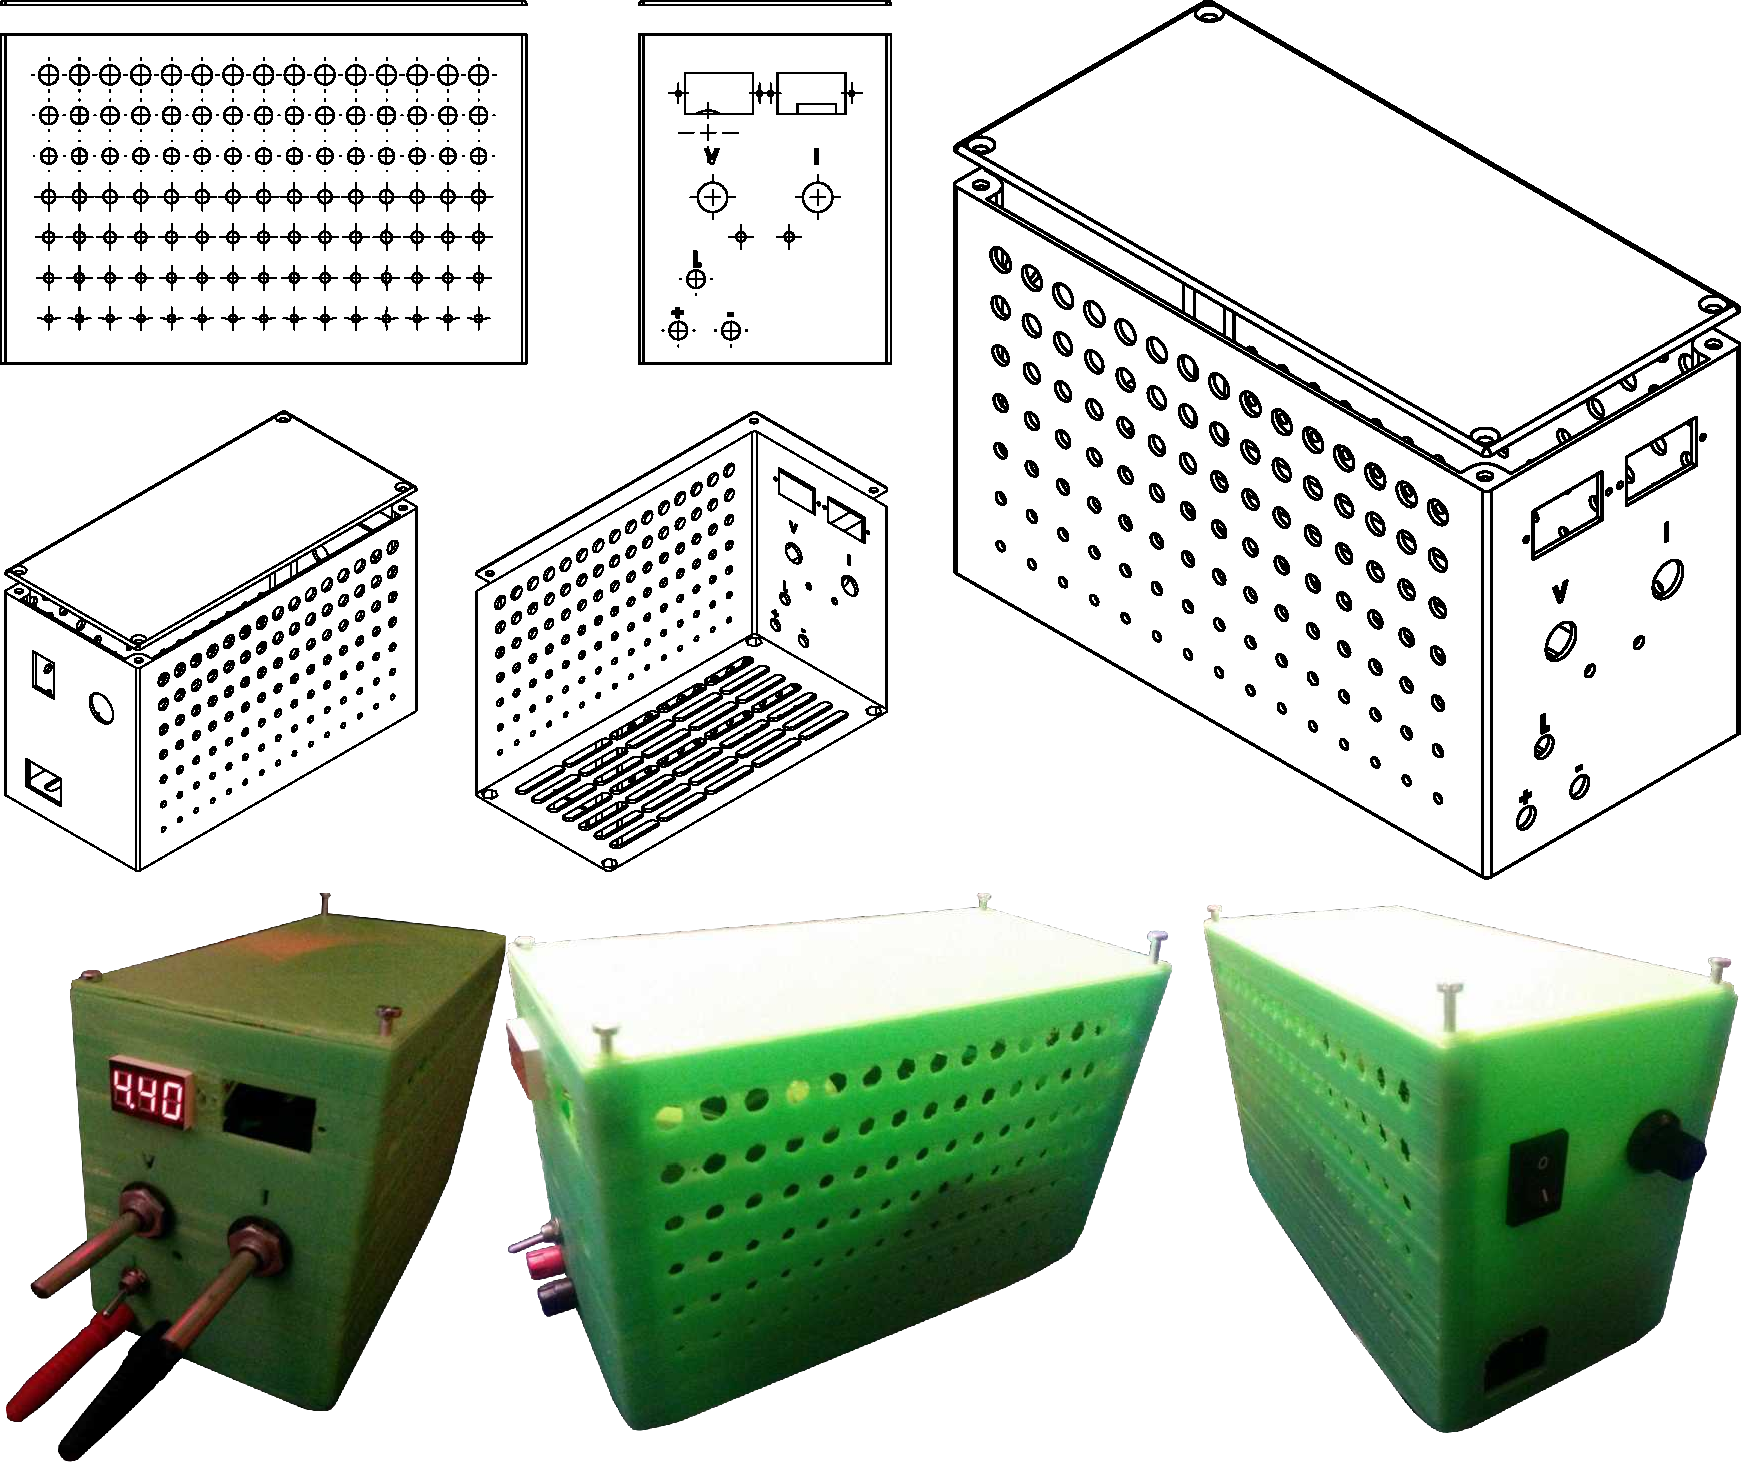
\includegraphics[width = 110mm]{resources/images/projects/solidworks/Bench_Power_Supply_Unit_Enclosure_Compressed.pdf} \\[1mm]
		\centering\small Laboratory bench power supply (SolidWorks)
	\end{figure}
	}}

\def\tooltipLabPowerBench{\parbox{110mm}{
	\textcolor{blue}{Laboratory DC power supply} \\[3mm]
	· \SI{24}{\volt} \SI{5}{\ampere} DC switching power supply \\[3mm]
	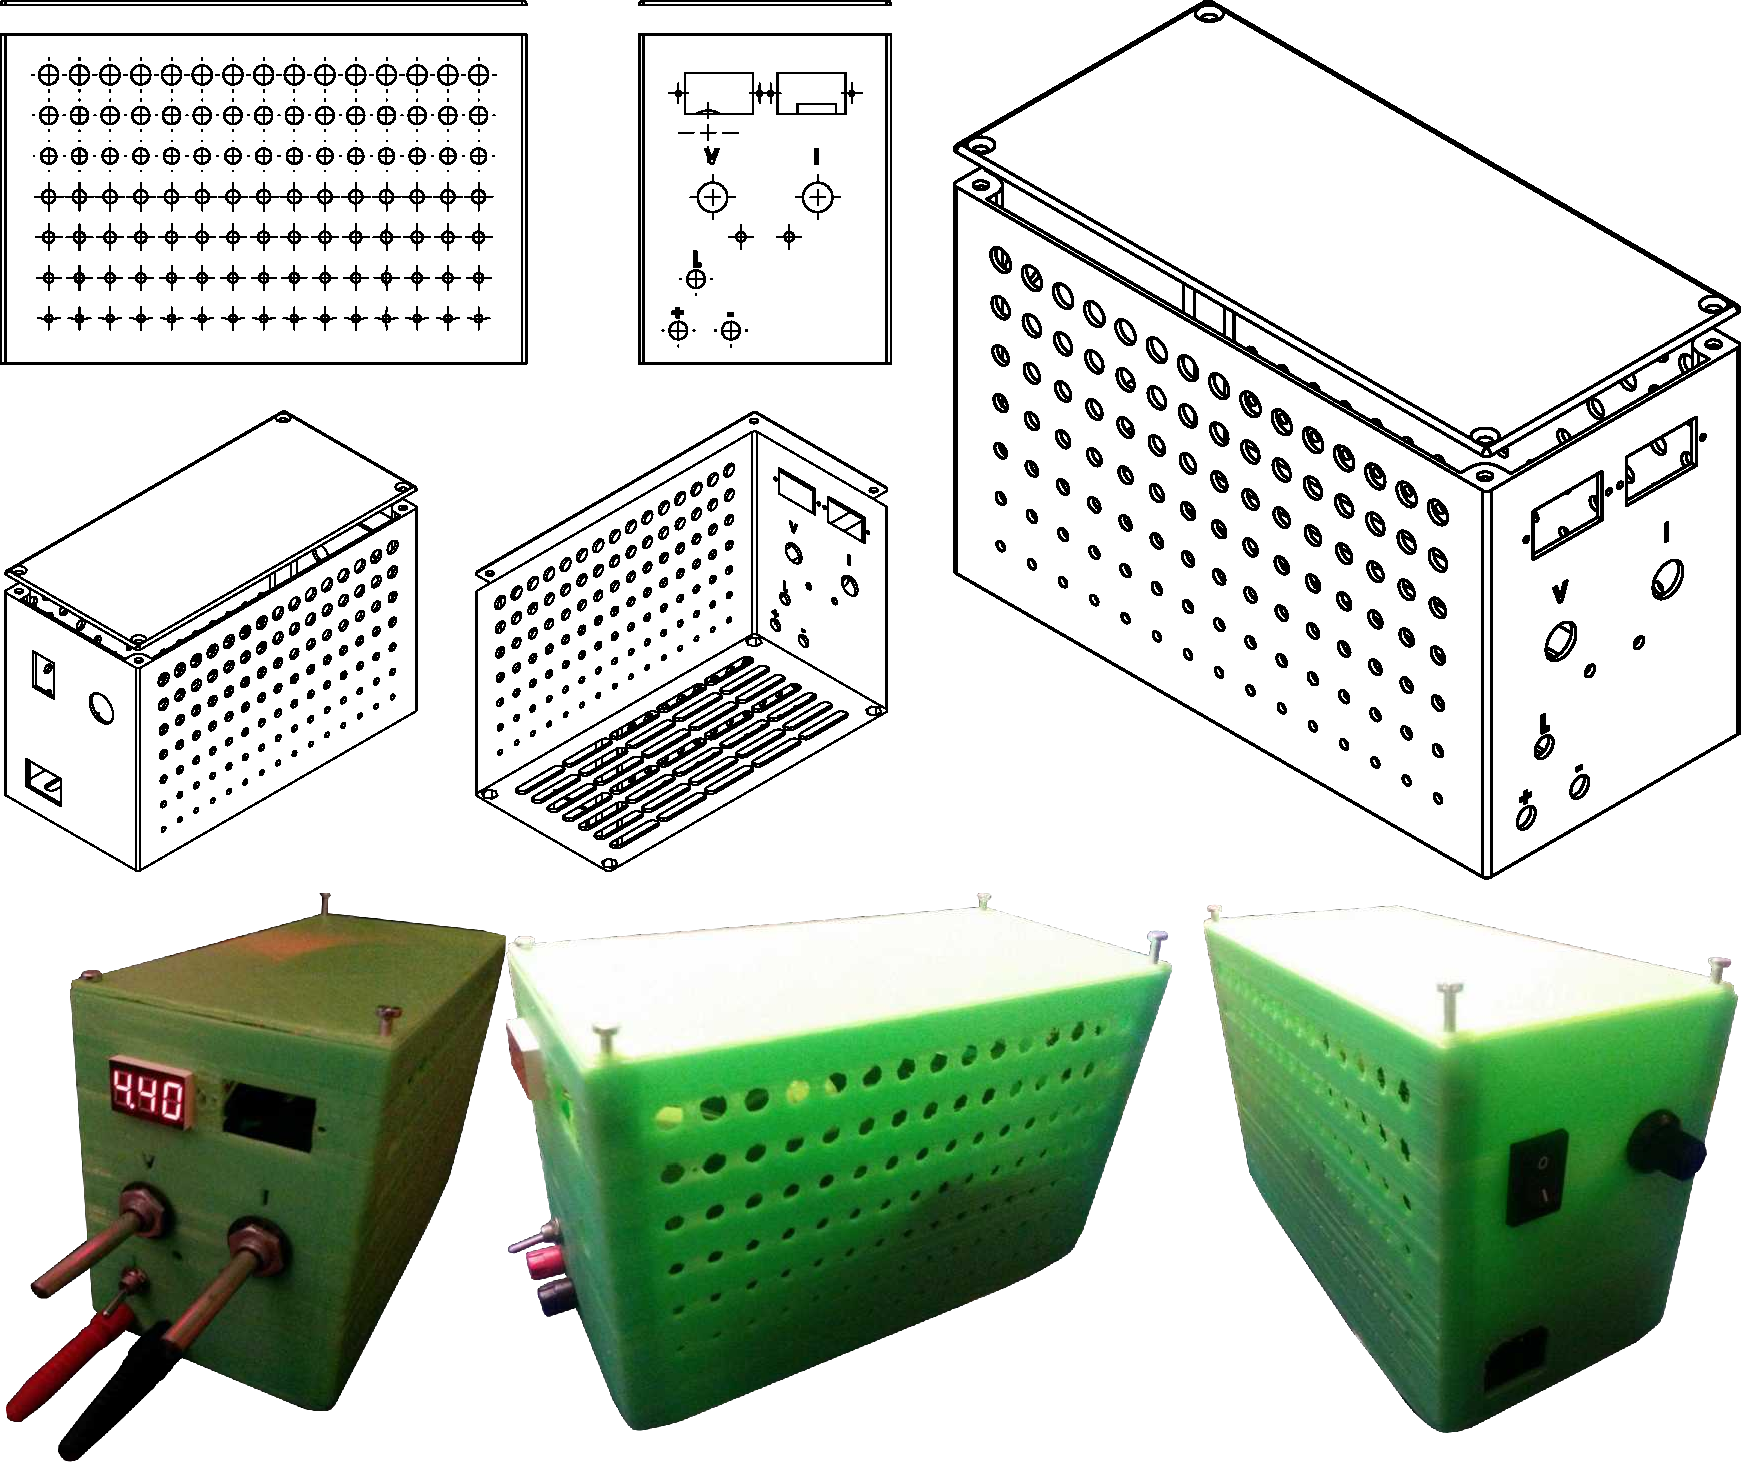
\includegraphics[width = 110mm]{resources/images/projects/solidworks/Bench_Power_Supply_Unit_Enclosure_Compressed.pdf} \\[1mm]
	}}

\def\tooltipLightningSwitch{\parbox{80mm}{
	\textcolor{blue}{IIoT intruder alarm and light switching} \\[3mm]
	· Sends an e-mail whenever occupancy is detected and the alarm is armed or the alarm has been enabled/disabled \\
	· Switches on and off (SSR relay) 2 AC lines (lightning) \\[3mm]
	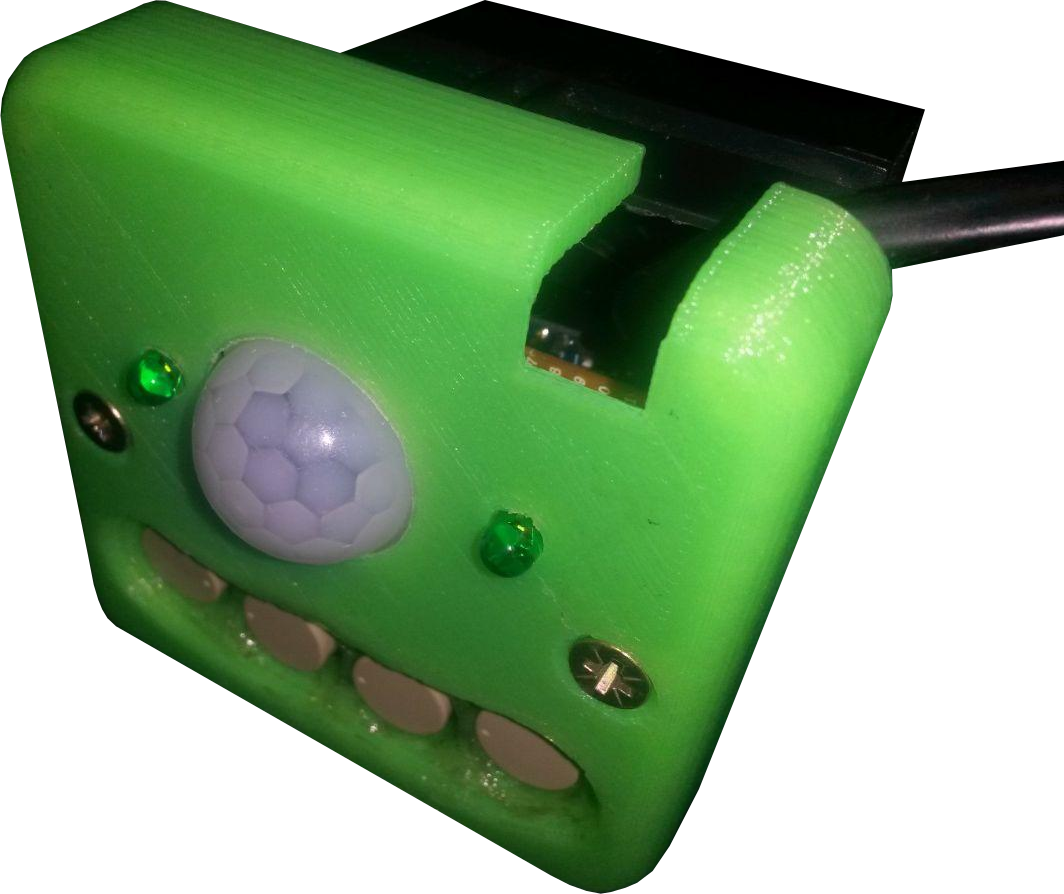
\includegraphics[width = 80mm]{resources/images/projects/iiot/panel_compressed.png} \\[1mm] 
	}}

\def\tooltipBachelorsDegreeThesis{\parbox{103mm}{

	\textcolor{tier@max}{Phython 1.0} \\[2mm]
	· Multijunction Photovoltaic Cells Simulator Implementation \\
	· Powered by Python 3.6 (GUI, data storage), C (numeric computing)
	· Thesis grade 9.8/10
	\vspace{-3mm}
	
	\begin{figure}[ht]
	\centering
	\parbox{\textwidth}{
		\parbox{.6\textwidth}{%
			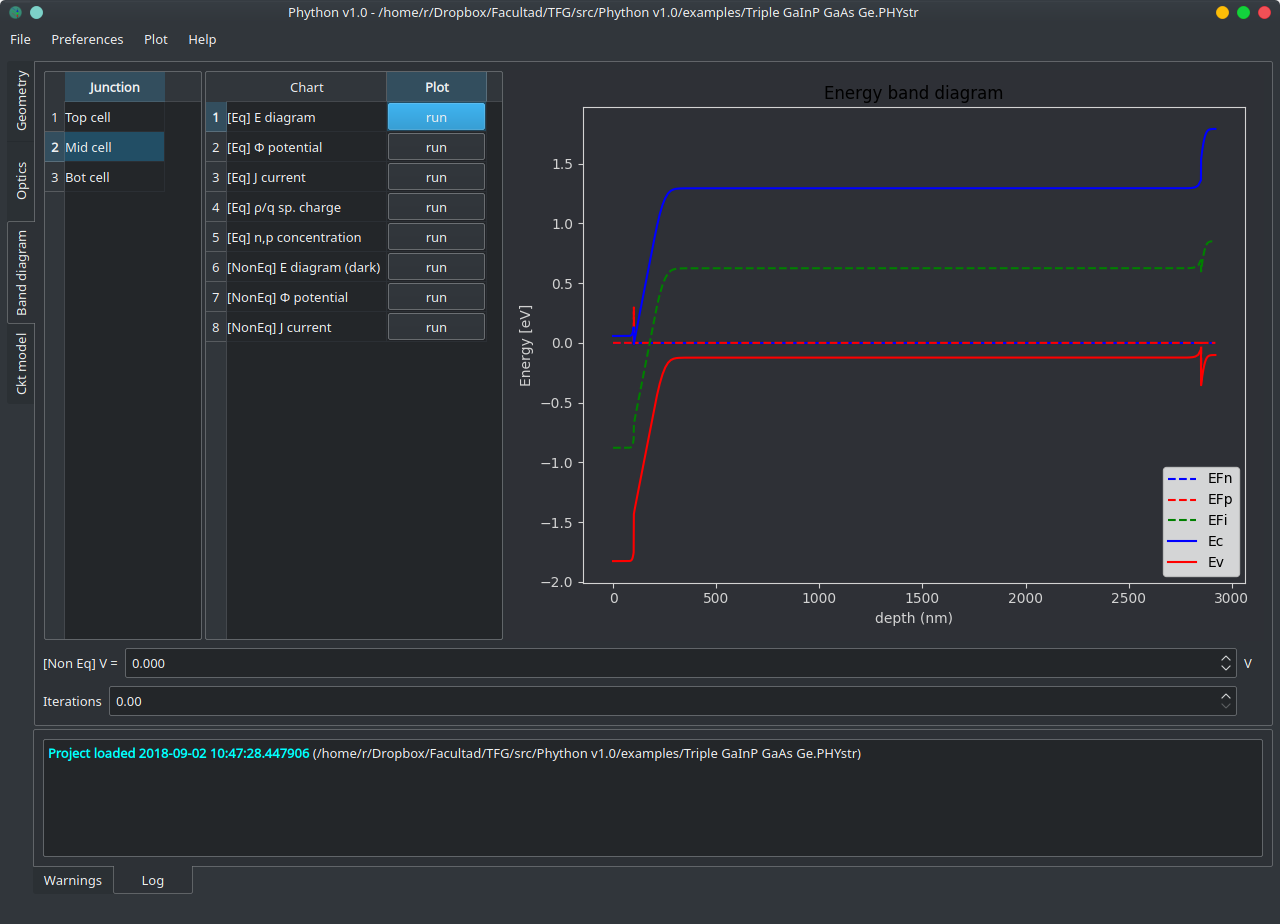
\includegraphics[height=50mm]{resources/images/projects/python/phython/bands.png} \\
			Band diagram (triple junction) simulation
			}
		\hspace{5mm}
		\parbox{.3\textwidth}{%
			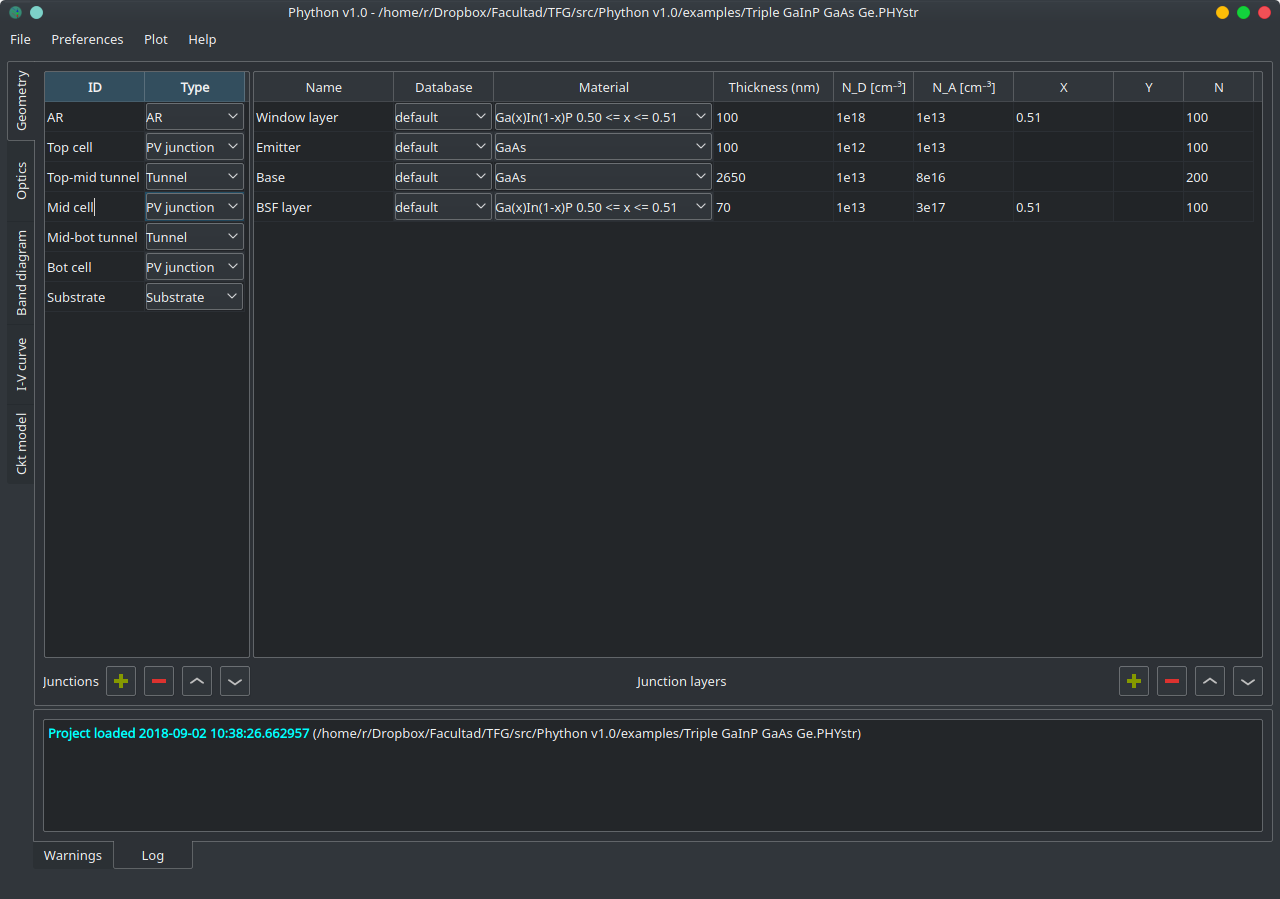
\includegraphics[height=21mm]{resources/images/projects/python/phython/layers.png} \\
			Multilayer definition \\[2mm]
			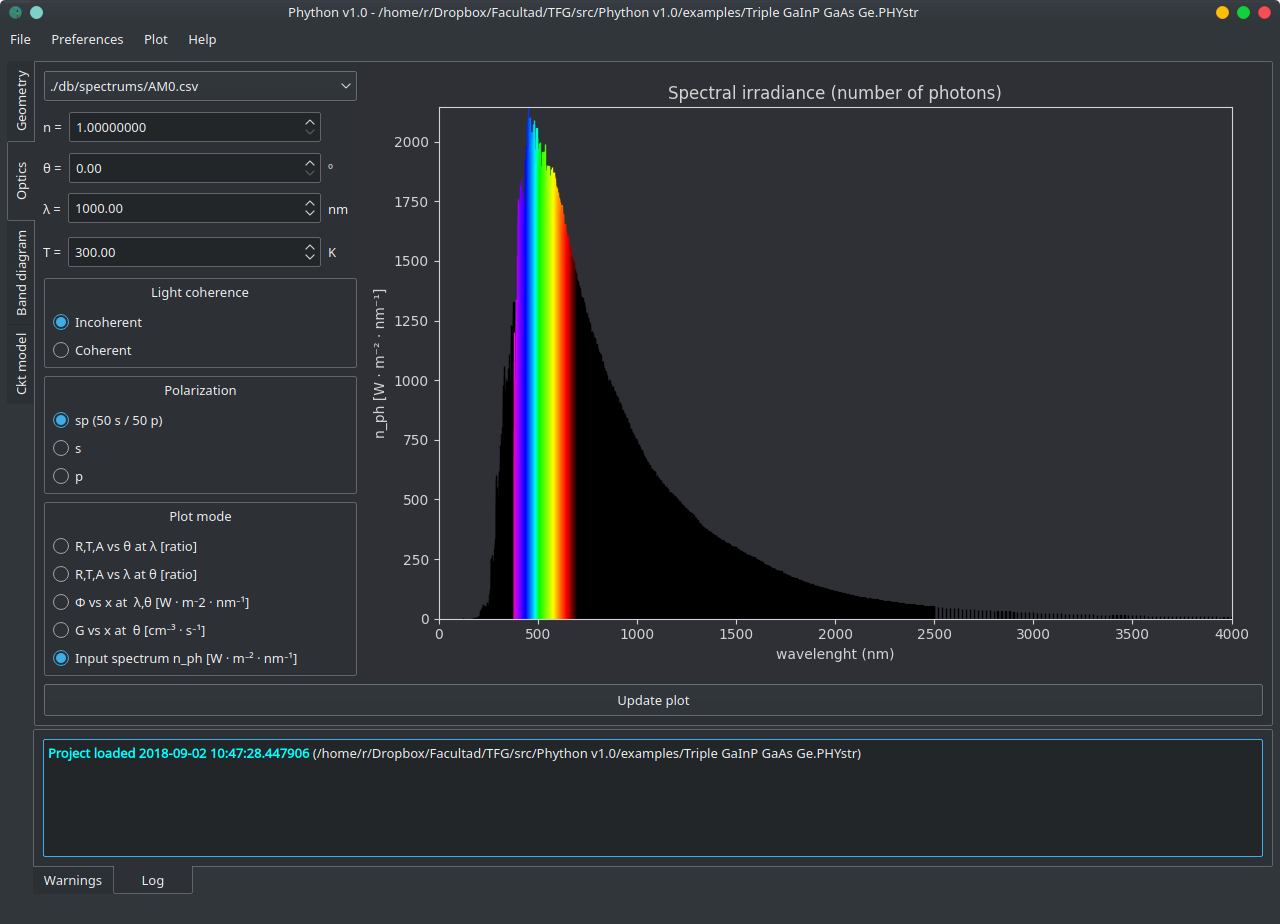
\includegraphics[height=21mm]{resources/images/projects/python/phython/optic.png} \\
			Spectrum input
			}
		}
	\end{figure}
	
	}}

\def\tooltipBachelorsDegreeSummary{\parbox{103mm}{

	\textcolor{tier@max}{Bachelor's degree in Industrial Electronic Engineering} \\[2mm]
	
	· Basics \\
	\phantom{hul} - Mechanics, Waves and Thermodynamics \\
	\phantom{hul} - Electromagnetism \\
	\phantom{hul} - Mathematics \\
	\phantom{hul} - Chemistry \\
	\phantom{hul} - Informatics \\
	\phantom{hul} - Technical Drawing and CAD \\
	
	· Electric \\
	\phantom{hul} - Electrical Technology I \\
	\phantom{hul} - Electrical Technology II \\
	\phantom{hul} - Machines and Mechanisms \\
	
	· Electronic \\
	\phantom{hul} - Electronic Components \\
	\phantom{hul} - Basic Electronics \\
	\phantom{hul} - Analog Electronics \\
	\phantom{hul} - Digital Electronics \\
	\phantom{hul} - Instrumentation Electronics \\
	\phantom{hul} - Sensors and Actuators \\
	\phantom{hul} - Power Electronics \\
	\phantom{hul} - Electronic Devices (Renewable Applications) \\
	\phantom{hul} - Energy Conditioning (Renewable Applications) \\
	\phantom{hul} - Signal Treatment and Transmission \\
	\phantom{hul} - Programmable Electronic Systems (FPGA) \\
	\phantom{hul} - Integrated Processors Theory \\
	\phantom{hul} - Design and Manufacturing of Integrated Circuits \\
	\phantom{hul} - Electronic Systems and Circuits (Biomedical Applications) \\
	
	· Industrial \\
	\phantom{hul} - Technical Thermodynamics and Flow Processes \\
	\phantom{hul} - Material Resistance \\
	\phantom{hul} - Science and Technology of Materials \\
	
	· Industrial Electronic \\
	\phantom{hul} - Control Fundamentals \\
	\phantom{hul} - Intelligent Control \\
	\phantom{hul} - System's Engineering \\
	\phantom{hul} - Automatisms \\
	\phantom{hul} - Industrial Communications \\
	\phantom{hul} - Prototyping and Electronic Testing \\
	
	· Management \\
	\phantom{hul} - Project Management \\
	\phantom{hul} - Enterprise Fundamentals \\
	\phantom{hul} - Production Management \\
	
	
	}}


% TODO
\def\tooltipLaTeX{\parbox{103mm}{%
	\textcolor{tier@med}{\LaTeX{}3} \\[2mm]
	· Class, package, command creation \\
	· Familiarized with PGF/TikZ \\
	· OCG (Optional Content Group): \\ 
	\phantom{hul} - Hyperlink referencing (\texttt{ocgbase}) \\
	\phantom{hul} - CAD drawings (\texttt{media9}) \\
	\phantom{hul} - Mouse over tooltips (Javascript + \texttt{ocgbase}) \\
	}}

%%%%%%%%%%%%%%%%%%%%%%%%%%%%%%%%%%%%%%%%%%%%%%%%%%%%%%%%%%%
%%%%%%%%%%%%%%%%%%%%%%%%% COURSES %%%%%%%%%%%%%%%%%%%%%%%%%
%%%%%%%%%%%%%%%%%%%%%%%%%%%%%%%%%%%%%%%%%%%%%%%%%%%%%%%%%%%

\def\tooltipOtherCourses{\parbox{103mm}{%
	\textcolor{tier@med}{Other courses} \\[2mm]
	· Organic Solar Cells, Technical University of Denmark (Coursera, audited)
	· Machine Design Part I, Georgia Institute of Technology (Coursera, audited)
	· Fundamentals of Audio and Music Engineering, University of Rochester (Coursera, audited)
	· Power Electronics (Coursera, audited, unfinished)
	}}

% TODO
\def\tooltipDevelopingIndustrialIoTSpecialization{\parbox{103mm}{%
	\textcolor{tier@max}{Developing Industrial IoT 3-course Specialization \hfill 29 hours} \\[2mm]
	\textcolor{tier@med}{Industrial IoT: Markets and Security \hfill 20 hours} \\[2mm]
	· Applications, market and solutions\\
	· Communication Protocols (Wireless) \\
	· Encryption: AES, PGP \\
	· Secure Systems: MD5, MAC \\
	· Key Generation \\
	· Key management, hardware and software protection \\[3mm]
	\textcolor{tier@med}{Project Planning and Machine Learning \hfill 9 hours} \\[2mm]
	· Project Management \\
	\phantom{A} \hfill Coursera (audited) \txtCourseraDifficulty{2}
	}}

% TODO
\def\tooltipCourseSolidWorks{\parbox{110mm}{
	\textcolor{blue}{SolidWorks} \hfill see GrabCAD 
\includegraphics[height=4mm]{resources/images/logos-circle/grabcad.pdf} \\[3mm]
	· Plastic part design
	\begin{figure}[H]
		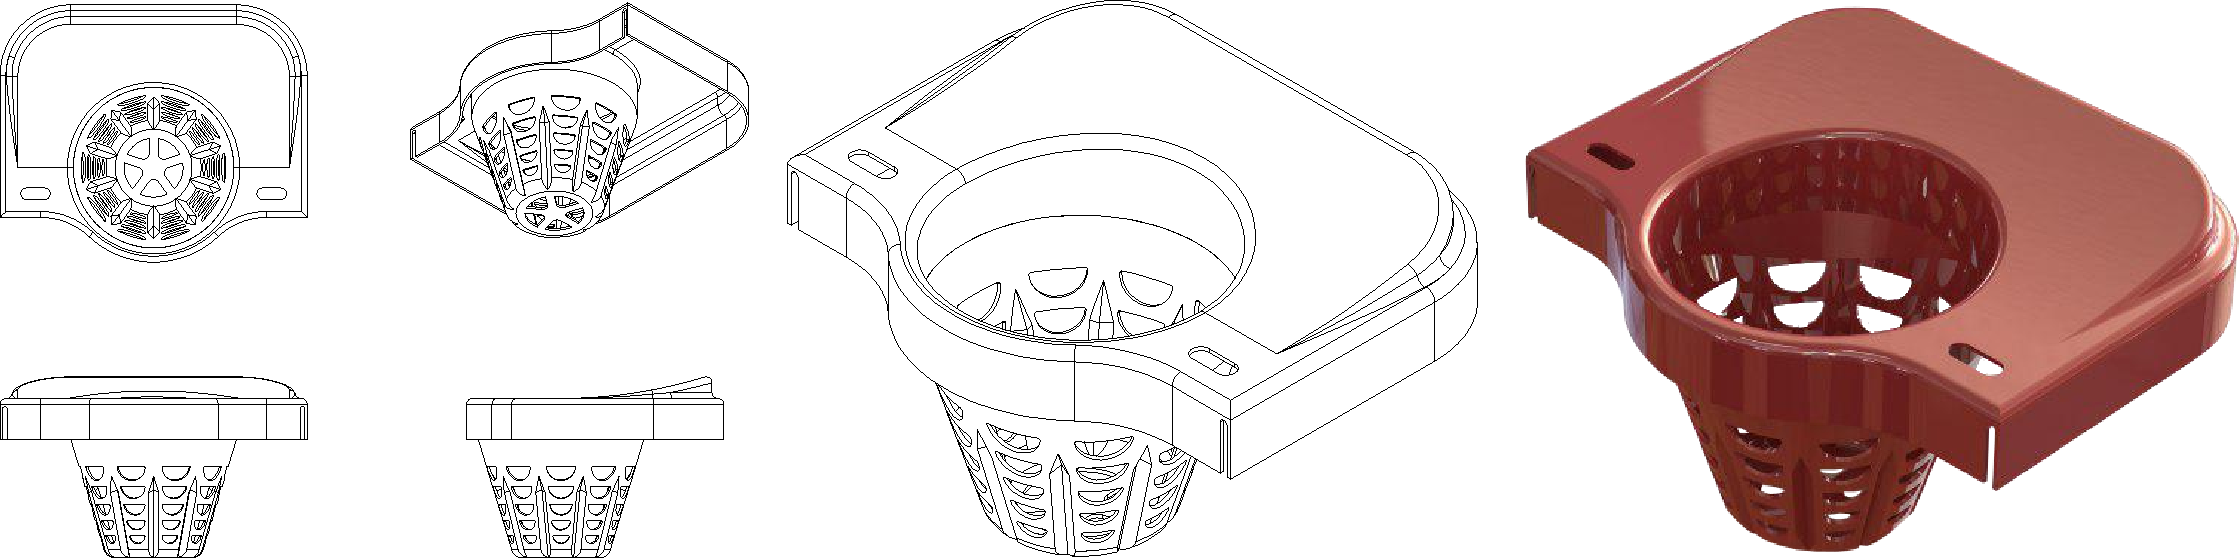
\includegraphics[width = 110mm]{resources/images/projects/solidworks/Mop_Wringer.pdf} \\[1mm]
		\centering\small Mop wringer (SolidWorks)
	\end{figure}
	}}

\def\tooltipSolidWorksCourse{\parbox{110mm}{
	\textcolor{blue}{SolidWorks} \\[3mm]
	· Part design (computation cost) \\
	· Structural simulation (security factor and mesh understanding) \\
	· Thermal simulation (transient and steady-state) \\
	· Flow simulation (cavitation) \\
	\begin{figure}
	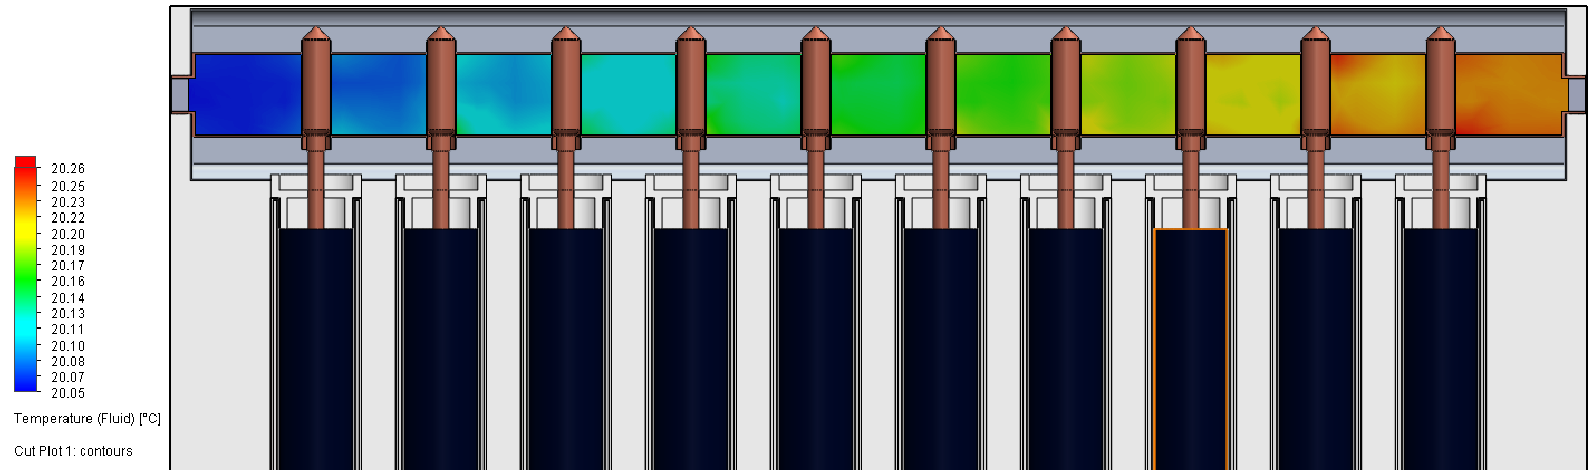
\includegraphics[width = 110mm]{resources/images/projects/courses/solidworks/final_project.png}
	\centering\small Final project: Simulation of evacuated tube flow
	\end{figure}
	}}

% TODO
\def\tooltipCourseraThreeDPrinting{\parbox{103mm}{%
	\textcolor{tier@max}{3D printing \hfill 44 hours} \\[2mm]
	\textcolor{tier@med}{3D printing: Revolution \hfill 8 hours} \\[2mm]
	\textcolor{tier@med}{3D printing: Applications \hfill 20 hours} \\[2mm]
	\textcolor{tier@med}{3D printing: Software \hfill 7/12 hours} \\[2mm]
	\textcolor{tier@med}{3D printing: Hardware \hfill 9 hours} \\[2mm]
	}}

% TODO
\def\tooltipSolarOne{\parbox{112mm}{
	\textcolor{blue}{Solar Photovoltaic Array Installation} \\
	· 800 W installation \\[3mm]
	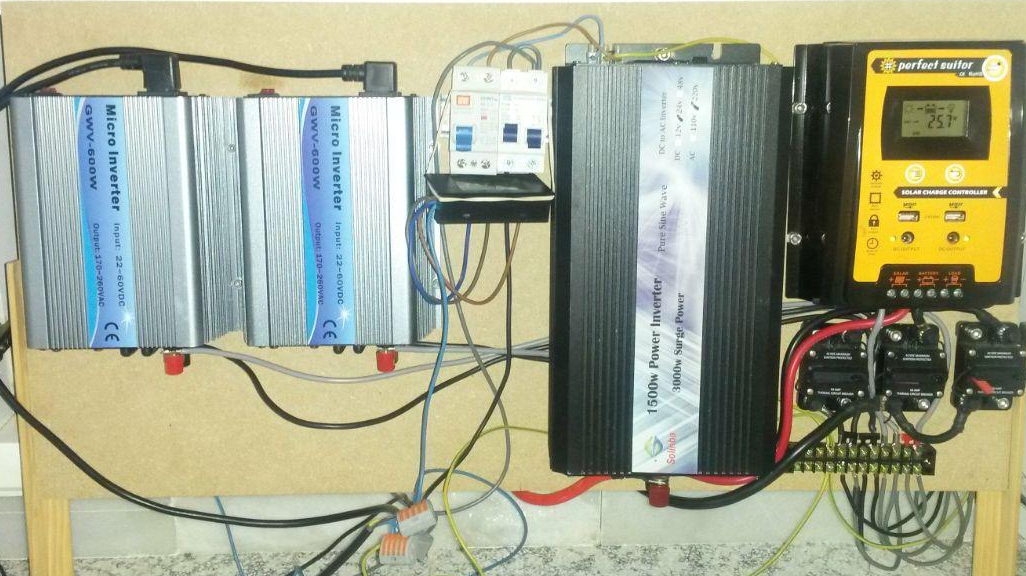
\includegraphics[width=112mm]{resources/images/projects/Solar/panel.png} \\[3mm]
	}}

% TODO
\def\tooltipMathCAD{\parbox{112mm}{
	\textcolor{blue}{MathCAD (PTC MathCAD Prime 4.0 and MathCAD 15} \\
	· Analog circuit tolerance optimization \\
	· Symbolic and parametric solutions \\
	· Data visualization \\
	· Importing and exporting
	}}



\begin{document}

\begin{page}


	% BODY %%%%%%%%%%%%%%%%%%%%%%%%%%%%%%%%%%%%%%%%%%%%%%%%%%%%%%%%%%%%%%%%%%%%%%

	\begin{layout}[fill = body@main@bkgd, size = 145mm, anchor = east]
	
		% Education
		\wgtIconAndText[text = body@sect@text, icon = body@sect@text]{resources/images/icons-circle/mortarboard.pdf}{\LARGE Education}
		
		\wgtVTimeline[draw = darkgray, right margin = 2mm]{{
			{2018}/{\textcolor{tier@max}{\large Industrial Electronic Engineering}}/{\small At University of Granada, Spain \\[1mm] \tooltip[background = tooltip@bkg, frame = tooltip@frm, underline = tier@max, dx = -40mm, dy = -240mm, sharp corner = northeast]{\textbf{Summary}}{\tooltipBachelorsDegreeSummary}: analog instrumentation, digital signals and systems, sensors and actuators, biomedical systems, power electronics, electric machines, mechanisms, semiconductor technology, robotics, mechanical design, materials science, microcontroller programming, PCB design, industrial communications... \\[1mm] \hreftooltip[sharp corner = northwest, background = tooltip@bkg, frame = tooltip@frm, underline = tier@max, dx = -3mm, dy = -92mm]{\small\textbf{Thesis}}{\tooltipBachelorsDegreeThesis}{https://drive.google.com/open?id=1W5290h3vZ74YY5a-EMViPIzxLgJladvF}: Multijunction Photovoltaic Cells Simulator Implementation in CPython
			}
			}}
		
		% Coursework
		\wgtIconAndText[text = body@sect@text, icon = body@sect@text, top margin = -2mm]{resources/images/icons-circle/books.pdf}{\LARGE Coursework}
		
		\wgtVTimeline[draw = darkgray, right margin = 2mm]{{
			{2020}/{\hreftooltip[dy = -90mm]{Deep Learning (work in progress)}{}{https://www.coursera.org/specializations/deep-learning}}/{\footnotesize deeplearning.ai (Coursera, audited)},
			{2019}/{\hreftooltip[underline = blue, dy = -90mm]{Developing Industrial IoT (2 courses) Specialization (29 h)}{\tooltipDevelopingIndustrialIoTSpecialization}{https://www.coursera.org/specializations/developing-industrial-iot}}/{\footnotesize University of Colorado Boulder (Coursera, audited)},
			{    }/{\textcolor{tier@med}{\hreftooltip[sharp corner = northwest, background = tooltip@bkg, frame = tooltip@frm, underline = tier@med, dx = -40mm, dy = -40mm]{Advanced English Certification (C1, Grade B)}{\parbox{40mm}{\textbf{Overall score} \hfill \textbf{193/210} \\ Reading \hfill 183/210 \\ Use of English \hfill 208/210 \\ Writing \hfill 186/210 \\ Listening \hfill 192/210 \\ Speaking \hfill 198/210}}{https://drive.google.com/open?id=1BnUG2yxlK6eBzjm_ZbpYfS26BZLTNP22}} }/{\footnotesize ESOL International Cambridge English Level 2},
			{2018}/{An Introduction to Programming the Internet of Things (IoT)}/{\footnotesize University of California, Irvine (Coursera, audited)},
			{2018}/{\hreftooltip[underline = black]{3D printing: revolution, applications, software and hardware (44 h)}{\tooltipCourseraThreeDPrinting}{https://www.coursera.org/learn/3d-printing-revolution}}/{\footnotesize University of Illinois at Urbana-Champaign (Coursera, audited)},
			{    }/{\textcolor{tier@med}{\hreftooltip[underline = blue]{Mechanical design and thermal, flow and structural simulation (72 h)}{\tooltipSolidWorksCourse}{https://formacion.fundacionugr.es/curso/diseno-mecanico-simulacion-termica-estructural-con-solidworks/}}}/{\footnotesize University of Granada}
			}}
		
		% Skillset
		\wgtIconAndText[text = body@sect@text, icon = body@sect@text, bottom margin = 3mm, top margin = -2mm]{resources/images/icons-circle/mortarboard.pdf}{\LARGE Skillset}
			
			\wgtText[align = justify, text = black, left margin = 5mm, bottom margin = 5mm]{
				\small
				\textbf{Computer-Aided design software}
					\begin{itemize}
						\item Parametric/feature modeling: \tooltip[background = tooltip@bkg, frame = tooltip@frm, underline = tier@med]{SolidWorks 2018}{\tooltipSolidWorks}, Autodesk Fusion 360
						\item EDA design: SPICE, SIMetrix/SIMPLIS, gEDA, Quartus II, EAGLE 2016
						\item CEM (Computational Electrodynamics): CST Microwave 2016
						\item Computation: MatLab r2016a, Maple 2016, Wolfram Mathematica 8.0
					\end{itemize}
				\textbf{Software}
					\begin{itemize}
						\item \tooltip[underline = blue]{Python}{\tooltipPython}, C/C++, Fortran90, Java, Lua, GNU Bash, JavaScript
						\item GNU/Linux OS user, familiarized with the Raspberry Pi 3B+ and pcDuino3
					\end{itemize}
				\textbf{Documentation}
					\begin{itemize}
						\item \tooltip[underline = black]{\LaTeX{}3}{\tooltipLaTeX}, \tooltip[underline = blue]{PTC MathCAD Prime 4.0, MathCAD 15}{\tooltipMathCAD}, various office suites
					\end{itemize}
				\textbf{Hardware}
					\begin{itemize}
						\item Embedded systems: Arduino-based boards, \tooltip[underline = black]{RTOS}{\tooltipRTOS}, \tooltip[underline = black]{Single-board computers}{\tooltipSBC}
						\item Communications: UART (GPS, GSM/GPRS...), SPI, I2C...
						\item Copper tubing soldering, PCB soldering, PCB etching
					\end{itemize}
				}
			
		% Meaningful projects
		\wgtIconAndText[text = body@sect@text, icon = body@sect@text, bottom margin = 3mm, top margin = -2mm]{resources/images/icons-circle/mortarboard.pdf}{\LARGE Meaningful projects}
			\wgtText[align = justify, text = black, left margin = 5mm, bottom margin = 5mm]{
				\small
				\textbf{Renewable energies}
					\begin{itemize}
						\item \tooltip[underline = blue]{800 W Solar photovoltaic array installation}{\tooltipSolarOne}
						\item Solar thermal system installation (evacuated tubes collector)
					\end{itemize}
				\textbf{Product design}
					\begin{itemize}
						%%%% OLD \item \tooltip[underline = blue]{Laboratory DC power supply}{\tooltipLabPowerBench}
						\item \tooltip[underline = blue]{IIoT (building automation): intruder alarm, light switching box and RFID lock}{\tooltipLightningSwitch}
					\end{itemize}
				}
				
	\end{layout}
	
	% SIDEBAR %%%%%%%%%%%%%%%%%%%%%%%%%%%%%%%%%%%%%%%%%%%%%%%%%%%%%%%%%%%%%%%%%%%
	
	\begin{layout}[fill = side@main@bkgd, size = 63mm, anchor = west]
	
		% Name	
		\wgtRightRounded[fill = side@sect@bkgd]{0.5cm}
		\wgtText[expand layout, text = side@sect@text, fill = side@sect@bkgd, minimum height = 1.6cm]
			{\Large Daniel Ríos Linares \\ \large Industrial Electronic Engineer}
		
		% Photo
		\wgtPhotoAndContact[bubble = side@dial@bubb]{resources/images/photo.png}{{
			\itmPhotoAndContactBubble{https://www.linkedin.com/in/danielrioslinares/}{resources/images/logos-circle/linkedin.pdf},
			\itmPhotoAndContactBubble{https://github.com/danielrioslinares/}{resources/images/logos-circle/github.pdf},
			\itmPhotoAndContactBubble{https://grabcad.com/daniel.rios.linares-1/models/}{resources/images/logos-circle/grabcad.pdf},
			\itmPhotoAndContactBubble{mailto:riv@hotmail.es}{resources/images/logos-circle/outlook.pdf},
			\itmPhotoAndContactBubble{https://t.me/riosL/}{resources/images/logos-circle/telegram.pdf}
			}}
		\wgtHSeparator
				
		% General info
		\wgtIconAndText[icon = side@info@icon, text = side@info@text]{resources/images/icons/birthday.pdf}{26/08/1994}
		\wgtIconAndText[icon = side@info@icon, text = side@info@text]{resources/images/icons/envelope.pdf}{\href{mailto:riv@hotmail.es}{\texttt{riv@hotmail.es}}}
		\wgtIconAndText[icon = side@info@icon, text = side@info@text]{resources/images/icons/phone.pdf}{\href{tel:+34665340504}{+34 665 34 05 04}}
		\wgtIconAndText[icon = side@info@icon, text = side@info@text]{resources/images/icons/geo.pdf}{Granada, Spain}
						
		% Goals
		\wgtRightRounded[fill = side@sect@bkgd]{0.5cm}
		\wgtText[expand layout, text = side@sect@text, fill = side@sect@bkgd, minimum height = 1.4cm]{\Large Goals}
		\wgtText[text = side@goal@text, align = justify, top margin = 2mm, bottom margin = 2mm]{\large To be part of meaningful engineering projects and become an experienced professional in the sector}
			
		% Languages
		\wgtRightRounded[fill = side@sect@bkgd]{0.5cm}
		\wgtText[expand layout, text = side@sect@text, fill = side@sect@bkgd, minimum height = 1.6cm]{\Large Languages}
			\itmTextAndHorizontalProgress[text = side@lang@text, fill = side@lang@fill, empty = side@lang@empt, top margin = 2mm, bottom margin = 2mm]{English}{85.0}
			\itmTextAndHorizontalProgress[text = side@lang@text, fill = side@lang@fill, empty = side@lang@empt, top margin = 2mm, bottom margin = 2mm]{Spanish}{100.0}
		
		% Interests
		\wgtRightRounded[fill = side@sect@bkgd]{0.5cm}
		\wgtText[expand layout, text = side@sect@text, fill = side@sect@bkgd, minimum height = 1.6cm]{\Large Interests}
		%%% OLD \wgtText[text = side@inte@text, align = justify, top margin = 2mm, bottom margin = 2mm]{
		%%% OLD 	· Computer programming \\
		%%% OLD 	· FOSS and OSHW \\
		%%% OLD 	· CNC machinery (3D printing)
		%%% OLD 	}
		\wgtDialRow[empty = side@dial@empt, fill = side@dial@fill, text = side@dial@text, minimum height = 11mm]{{
			{\small SolidWorks}/{resources/images/logos-circle/solidworks.pdf}/82/{\tooltipCourseSolidWorks},
			{\small IoT}/{resources/images/icons-circle/brain.pdf}/90/{},
			{\small 3D printing}/{resources/images/icons-circle/3dprinter.pdf}/80/{\tooltipThreeDPrinting}
			}}
		\wgtDialRow[empty = side@dial@empt, fill = side@dial@fill, text = side@dial@text, minimum height = 11mm]{{
			{\small Computation}/{resources/images/icons-circle/computer.pdf}/92/{},
			{\small Power Elec.}/{resources/images/icons-circle/power.pdf}/87/{},
			{\small Python}/{resources/images/logos-circle/python.pdf}/94/{\tooltipPython}
			}}		
		
		% Interests
		\wgtRightRounded[fill = side@sect@bkgd]{0.5cm}
		\wgtText[expand layout, text = side@sect@text, fill = side@sect@bkgd, minimum height = 1.6cm]{\Large Hobbies}
		\wgtText[text = side@inte@text, align = justify, top margin = 2mm, bottom margin = 2mm]{
			· Guitar playing \\
			· Cooking \\
			· Travelling \\
			· Technical writing
			}
		
	\end{layout}
	
	\begin{layout}[fill = side@sect@bkgd, size = 2mm, anchor = west]
	\end{layout}
	
	\begin{layout}[fill = side@sect@bkgd!10, size = 1mm, anchor = west]
	\end{layout}
	
	
	
	
	
	
	
\end{page}




\end{document}
